\chapter{引言}
本章节主要介绍课题的研究背景与意义、研究内容与成果，以及论文的组织结构。

\section{背景与意义}
容器技术通过内核级资源隔离与标准化的镜像分发机制，极大地优化了微服务应用的生命周期管理。作为容器编排领域的核心基础设施，Kubernetes 提供的分布式容器编排能力有效支撑了复杂业务的部署与扩展\cite{kubernetes2024,alibaba2024}。为满足多样化的服务治理需求，现代 Kubernetes 集群需深度集成云原生计算基金会(CNCF)开源生态中的第三方应用，各类组件通过基于角色的访问控制 (RBAC) 机制\cite{ferraiolo1995role}获取集群资源访问权限。这些第三方应用的使用在赋能业务的同时也化引入了潜在的攻击面，特别是在多租户场景下，过度权限配置\cite{yang2023take}、内部权限管理缺陷、敏感信息泄露、网络隔离缺失等多维因素可能带来权限提升风险，对云原生系统的整体安全构成系统性威胁。
\begin{figure}[htbp]
    \centering
    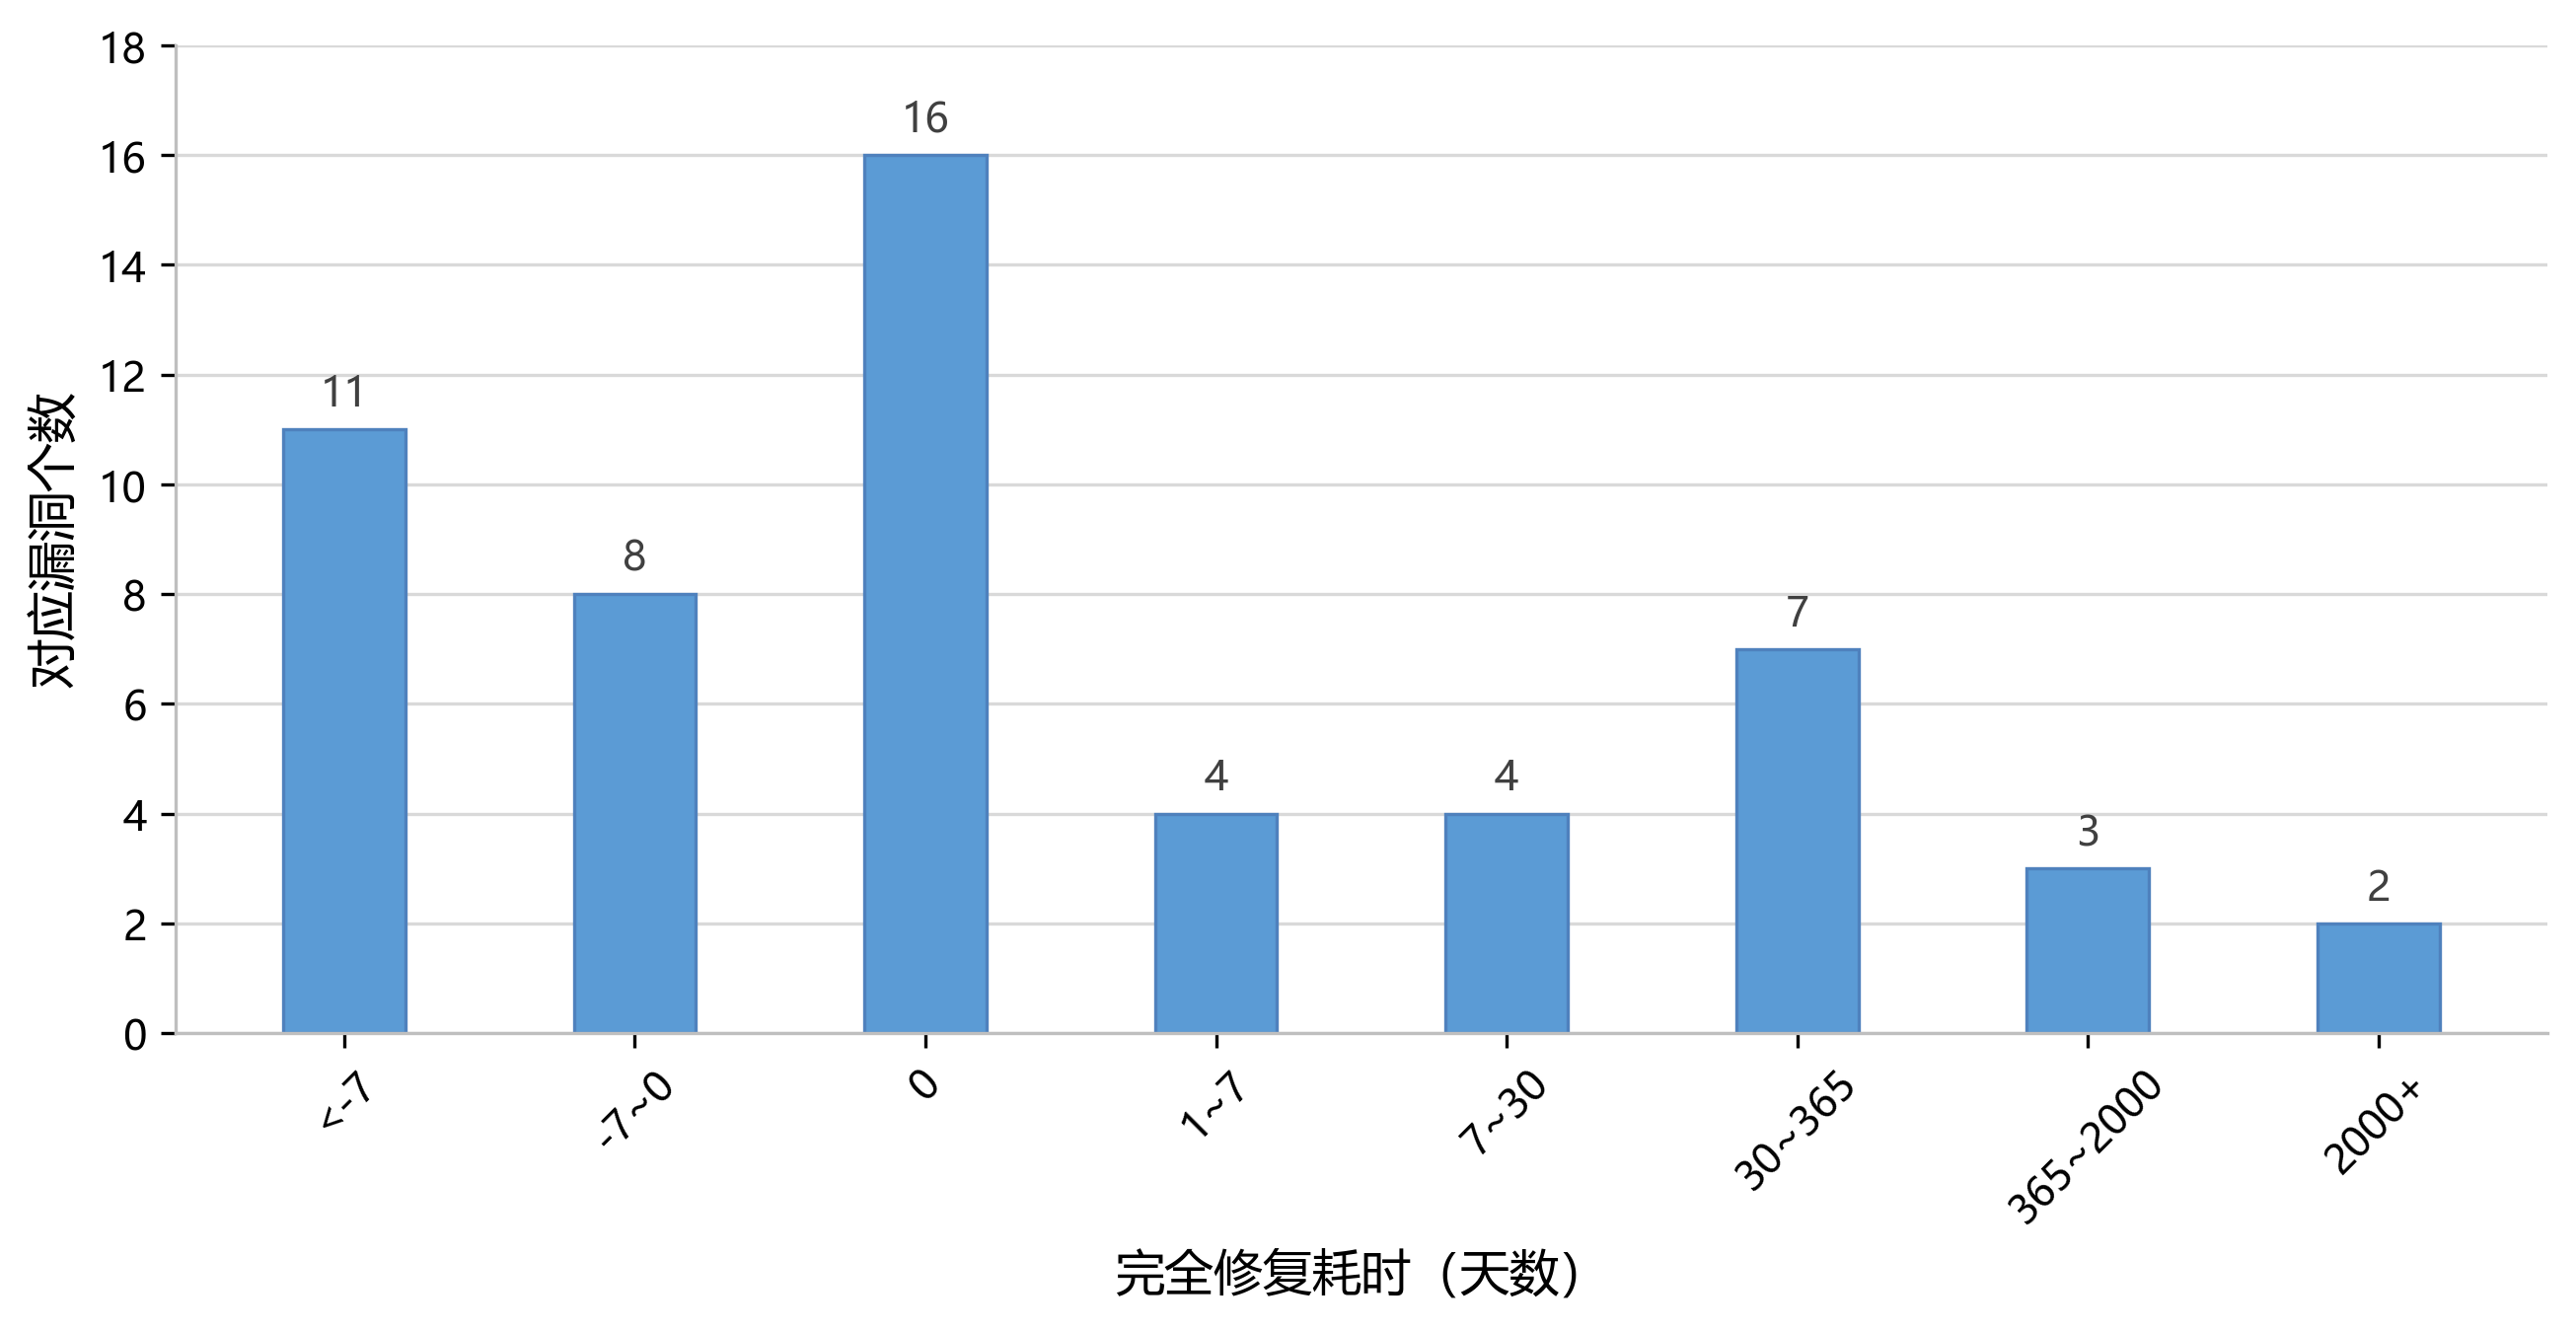
\includegraphics[width=0.8\textwidth]{images/cve-pub.png}
    \caption{云原生环境下权限提升漏洞的修复时间分布}\label{fig:patch-window}
\end{figure}

云原生第三方开源应用的权限提升漏洞从披露到修复通常面临显著的响应滞后。根据本文统计的2020年至2025年间55个云原生权限提升漏洞样本的统计，有30.4\%漏洞在披露后存在较长的攻击窗口期(见图~\ref{fig:patch-window})。开源应用官方补丁的发布、验证与分发存在相应周期管理失职会带来攻击窗口；进一步的，由于生产环境组件组合复杂且兼容性要求高，用户往往难以及时完成受影响组件的升级。在补丁尚未就绪或升级受阻的阶段，企业亟需一种可快速下发、可验证且可回滚的临时防控措施，通过压制攻击路径来降低风险暴露面。


\section{内容与成果}
基于上述现实需求，本文聚焦于云原生权限提升漏洞在补丁窗口期内的动态防控技术。通过分析漏洞公告与多维可追溯上下文，基于大语言模型构建多智能体协同的安全策略生成系统，自动化生成并筛选针对性的临时防控策略。从防控机制的作用维度考量，本文将云原生环境下的动态控制手段归纳为\textbf{监控策略}与\textbf{防护策略}两个互补层次：其中监控策略侧重运行时异常行为的感知与取证，防护策略侧重事前阻断与攻击面收敛。具体可落地控制点包括： 
\begin{itemize} 
    \item \textbf{防护策略层}：
    \begin{itemize}
        \item \textit{准入控制与配置约束}：通过 OPA/Gatekeeper\cite{opa2025} 或 Kyverno\cite{kyverno2025} 等准入控制器，在资源对象持久化前对特权容器、危险路径挂载及异常 RBAC 绑定等高风险配置实施\textbf{强制阻断}。
        \item \textit{网络隔离与连通收敛}：基于 NetworkPolicy 构建微隔离边界，将工作负载间可达性收敛至最小必要集合，从而抑制横向移动与数据外传路径。
        \item \textit{权限与配置动态加固}：面向漏洞利用路径，通过收紧 RBAC 授权边界、移除冗余权限以及调整容器运行时安全上下文，压缩攻击成功概率。
    \end{itemize}
    \item \textbf{监控策略层}：
    \begin{itemize}
        \item \textit{运行时行为监测}：基于 Falco\cite{falco2025} 等系统调用层监控工具，对异常系统调用、特权提升行为及敏感文件访问进行\textbf{实时告警与取证}，并可结合响应流程抑制影响扩散。
    \end{itemize}
    \item \textbf{防测一体工具}：
    \begin{itemize}
        \item \textit{Cilium Tetragon}\cite{tetragon2025}：基于 eBPF 的安全观测与运行时强制执行工具，兼具\textbf{监控策略}（进程执行、系统调用、I/O活动的实时检测）与\textbf{防护策略}（内核层面的策略过滤与阻断）能力，实现从感知到响应的闭环防护。
    \end{itemize}
\end{itemize}

\begin{figure}[htbp]
    \centering
    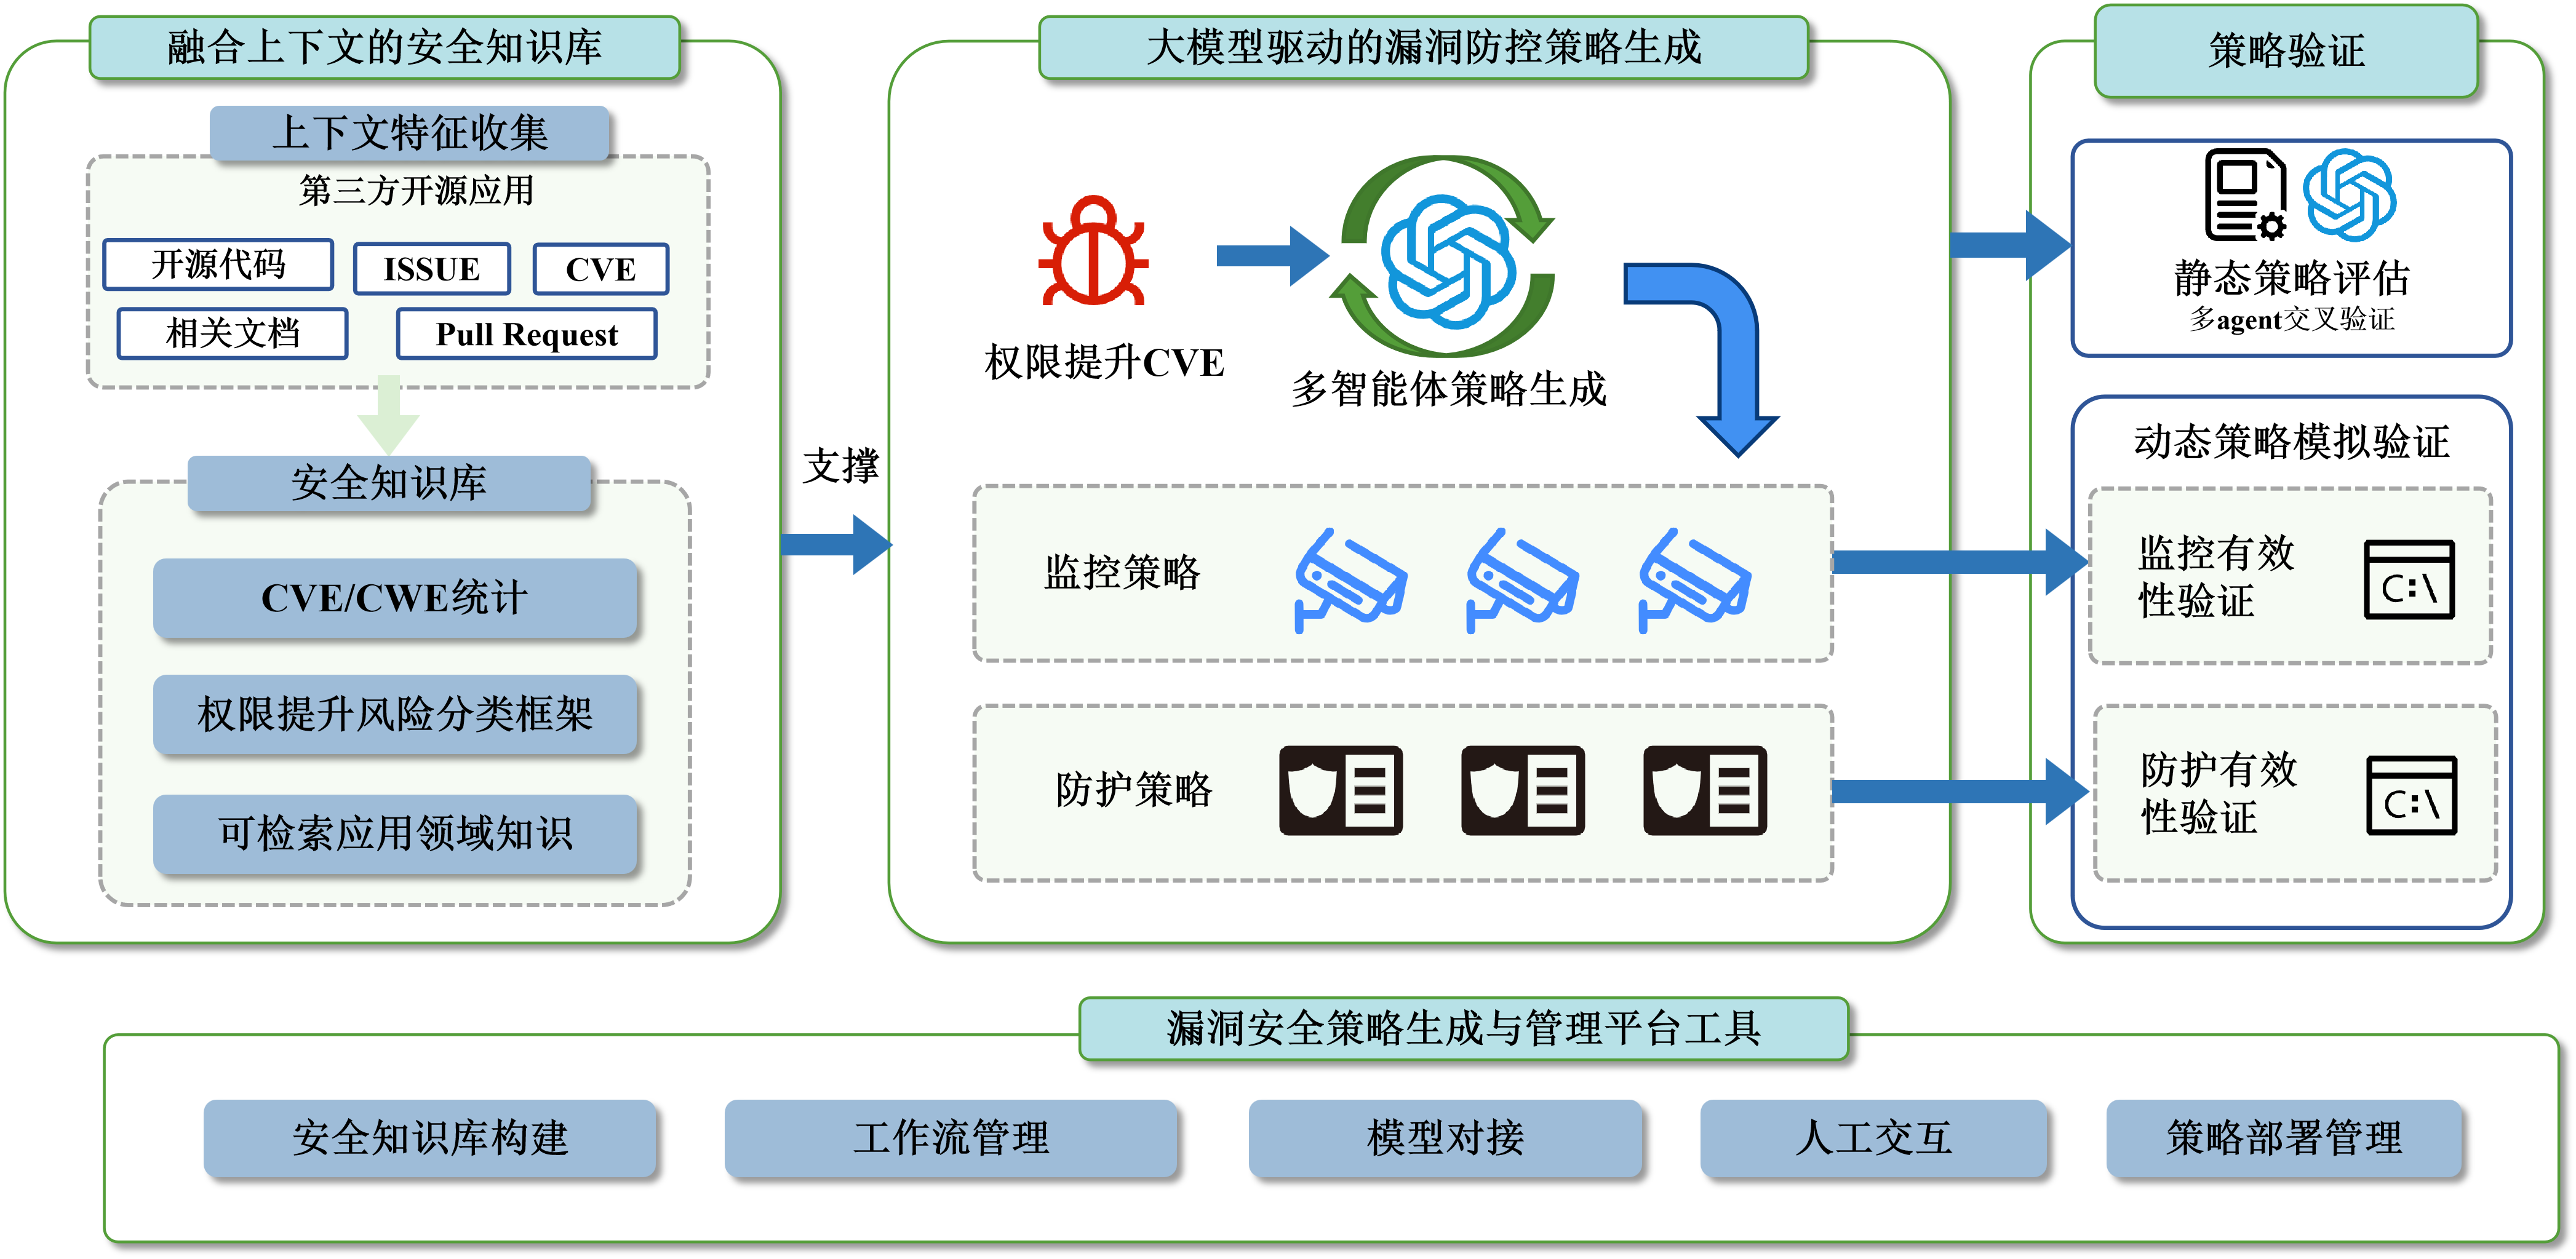
\includegraphics[width=0.98\textwidth]{images/总体框架.png}
    \caption{基于大语言模型的多 Agent 漏洞临时防控总体框架}\label{fig:overall-framework}
\end{figure}

如图~\ref{fig:overall-framework}所示，本文提出的自动化临时防控框架围绕安全知识库、策略生成与策略验证形成闭环，具体研究点包括：
\begin{itemize}
    \item \textbf{融合上下文的安全知识库构建}：面向云原生第三方开源应用场景，融合漏洞公告、开源代码与社区协作信息等多源上下文，形成可追溯的漏洞事实依据与可检索的领域知识，并沉淀面向权限提升风险成因的分类框架。
    \item \textbf{多智能体协同的防控策略生成}：以权限提升类 CVE 为输入，在知识库支持下组织多智能体协同生成候选策略集合，涵盖监控策略与防护策略两类控制目标，输出可执行的策略草案。
    \item \textbf{安全策略筛选与验证}：结合静态策略评估与动态模拟验证，对候选策略进行有效性与安全性筛选，保证策略具备可部署、可验证与可回滚的工程可用性。
    \item \textbf{平台化工具支撑}：提供知识库维护、工作流编排、模型对接与策略部署管理等能力，支撑策略生成与验证过程的持续迭代。
\end{itemize}





\section{论文组织结构}

全文结构如下：第\ref{chap:background}章介绍相关概念、技术与国内外研究现状；第\ref{chap:method}章给出面向云原生权限提升漏洞的智能防控技术体系；第\ref{chap:system}章描述漏洞防控系统设计与实现；第\ref{chap:experiment}章呈现实验设置与结果；第\ref{chap:case}章给出案例分析；第\ref{chap:conclusion}章总结与展望。